\documentclass[]{article}
\usepackage[nonumber]{cuisine}
\usepackage[]{graphicx}
%opening
\title{}
\author{}

\begin{document}

\begin{recipe}{Pork-Taro Spring Roll}{}{Makes About 50 small egg rolls.}
	\ingredient[1]{lb}{Taro}
	\ingredient[1]{lb}{Carrot}
	Shred carrots and taro. 
	\ingredient[1]{large}{Egg}
	Separate and set whites aside. 
	\ingredient[1]{lb}{Ground Pork}
	\ingredient[1]{tbsp}{Salt}
	\ingredient[1]{tbsp}{Ground Black Pepper}
	Combine with vegetables and egg yolk in large bowl.
	\ingredient[50]{}{TYJ Spring Roll Pastries} 
	Roll spring rolls and deep-fry in batches at $350-375^\circ$F until golden brown. Use a food thermometer to confirm that internals are $165^\circ F$.
	\ingredient[]{}{}
\end{recipe}

\begin{figure}[h]
	\center
	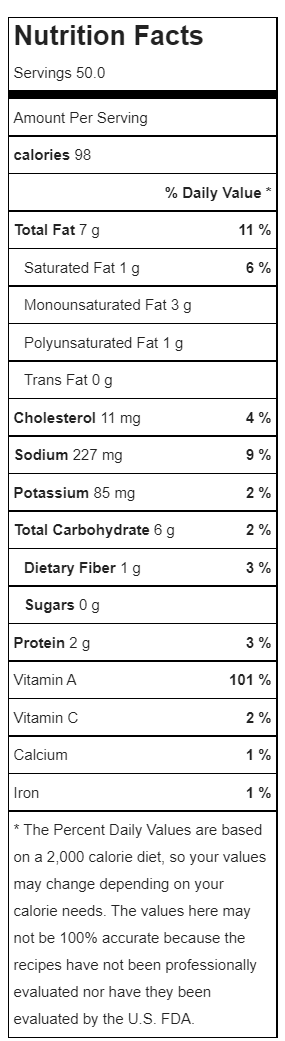
\includegraphics[width=0.25\linewidth]{MFP.png}
\end{figure}
\end{document}
